\documentclass[11pt,a4paper,oneside]{article}
\usepackage[dutch]{babel}
\usepackage{amsmath}
\usepackage{graphicx}
\usepackage{tikz}
\usepackage{fancyhdr}
\usepackage{dsfont}
\usepackage{parskip}
\usepackage{epstopdf}
\usepackage{listings}
\usepackage{color}
\definecolor{lichtgrijs}{gray}{0.95}
\usepackage{cite}
\usepackage[nottoc]{tocbibind}
\usepackage[T1]{fontenc}
\usepackage[light,math]{iwona}
\usepackage{pgfplots}
%\pgfplotsset{compat=newest}
\usepackage{subfig}
\usepackage{textcomp}
\usetikzlibrary{arrows,automata}
\usepackage{float}
\usepackage{longtable}
\usepackage{titling,enumitem}
\usepackage{a4wide}
\usepackage{amssymb}
\usepackage{rotating}
\usepackage{listings}
\usepackage[top=1.1in, bottom=1.2in, left=1.1in, right=1.1in]{geometry}
\usepackage{array}
\usepackage{titling}
\usepackage{blindtext}
\usepackage{chngpage}
\usepackage{calc}
\definecolor{lightgray}{gray}{0.8}
\newcolumntype{L}{>{\raggedleft}p{0.50\textwidth}}
\newcolumntype{R}{p{0.8\textwidth}}
\newcommand\VRule{\color{lightgray}\vrule width 0.5pt}
\usepackage{color, colortbl}
\definecolor{Gray}{gray}{0.9}
\definecolor{dkgreen}{rgb}{0,0.6,0}
\definecolor{gray}{rgb}{0.5,0.5,0.5}
\definecolor{mauve}{rgb}{0.58,0,0.82}
\definecolor{ugentblue}{rgb}{0.05,0.18,0.37}
\usepackage{import}
\usepackage[T1]{fontenc}
\begin{document}

%\newgeometry{top=0.8cm, right=1.70cm, left=1.7cm}
\begin{titlepage}

\thispagestyle{fancy}
\fancyhf{}
\fancyfoot[L]{}
\begin{figure}[!ht]
  \begin{adjustwidth}{-\oddsidemargin-1in}{-\rightmargin}
    \centering
    
\includegraphics[width=\paperwidth]{banner}
  \end{adjustwidth}
\end{figure}
\vspace{-0.2em}
\begin{center}
\vspace{5cm}
\Huge \textbf{Vakoverschrijdend Project: team Edran\\ Rapport episode 3}\\
\vspace{6.0cm}
\large
\begin{tabular}{L! {} R}
& {\LARGE\bf Team Edran} \\
& \\
& {\bf Steven De Blieck} \\
& {\bf Laurens De Graeve} \\
& {\bf Bart Middag} \\
& {\bf Wouter Pinnoo} \\
& {\bf Robin Praet} \\
& {\bf Stijn Seghers} \\
& {\bf Wouter Termont} \\
& {\bf Gilles Vandewiele} \\
\end{tabular}
\end{center}
\end{titlepage}
%\restoregeometry
\newpage

\fancyheadoffset[RO,LE]{0in}
\fancypagestyle{plain}{
\fancyhead[L]{Rapport episode 3}
\fancyhead[R]{Team Edran}
\fancyfoot[L]{}
\fancyfoot[R]{\thepage}}

\fancyhead[L]{Rapport episode 3}
\fancyhead[R]{Team Edran}
\fancyfoot[L]{}
\fancyfoot[C]{\thepage}
\pagestyle{fancy}
\tableofcontents
\newpage

\setcounter{section}{0}
\setcounter{subsection}{0}
\part{Verwachte functionaliteiten}
\begin{itemize}
	\item	Bewijsmateriaal moet kunnen upgeload worden naar de website. Hierna kan men dit ook verwijderen, of hier nog bewijsmateriaal aan toevoegen.
		Hierbovenop moet een beheerder de correctheid van het bewijsmateriaal controleren en vervolgens accepteren of goedkeuren.
	\item   Wanneer er zich een bepaalde gebeurtenis voordoet, wordt de gebruiker hier van op de hoogte gehouden aan de hand van een notificatiesysteem. Het is de beheerder
		die specifieert bij welke gebeurtenissen een notificatie verstuurd moet worden.
	\item   Van verschillende pagina's moet een rapport kunnen gegenereerd worden.
	\item 	Er moeten schadedossiers kunnen aangemaakt en gewijzigd worden door een beheerder.
	\item   Een beheerder kan een gebruiker tijdelijk blokkeren van de website.
	\item	Een superuser kan machtigingen (bv het goed- en afkeuren van bewijsmateriaal) toewijzen aan een beheerder.
	\item	Een autoeigenaar moet autogebonden gegevens kunnen inbrengen (zoals bv carwash).
	\item	Bij registratie kan een autoeigenaar zijn auto toevoegen aan het systeem. Het is tenslotte de beheerder die dit goed- of afkeurt.
\end{itemize}

\setcounter{section}{0}
\setcounter{subsection}{0}
\part{Episode IV}
De volgende episode wordt voorbehouden voor code refactoring, bug fixes en implementatie van details.

\setcounter{section}{0}
\setcounter{subsection}{0}
\part{Bewijsmateriaal}
\section{Usescases}
\subsection{Toevoegen van bewijsmateriaal}
Het toevoegen van bewijsmateriaal kan zich voordoen in twee verschillende situaties:
\begin{itemize}
 \item Een gebruiker heeft tijdens het maken van een rit een kost gemaakt (bv. carwash). Hiervoor moet bewijsmateriaal geuploaded worden bij het inbrengen van de ritgegevens.7
 \item Een autobeheerder heeft een kost gemaakt (zonder het maken van een rit). Het bewijsmateriaal wordt geuploaded bij het inbrengen van autogebonden gegevens (onder het tabblad 'Autobeheer')
\end{itemize}
De gebruiker selecteert de gemaakte kost uit een lijst en voert het bedrag in. Wanneer de gebruiker op een knop 'Upload!' klikt, zal een bestandsverkenner verschijnen. Hier selecteert de gebruiker het gewenste bestand en klikt op toevoegen. 
Op de pagina wordt de foto nog eens getoond, zo dat de gebruiker kan controleren of het de juiste foto is. Optioneel kan ook nog commentaar toegevoegd worden.

\subsection{Beheren van bewijsmateriaal}
Zelf na het inbrengen van autogebonden gegevens of ritgegevens kan een gebruiker nog bewijsmateriaal toevoegen aan het systeem. Als de gebruiker pas later
beseft dat hij verkeerd bewijsmateriaal toegevoegd heeft, kan hij dit nog verwijderen.

\subsection{Verifi\"{e}ren van bewijsmateriaal}
Om fraude tegen te gaan, moet vooraleer een bewijsmateriaal als 'correct' wordt beschouwd eerst een goedkeuring door de beheerder gebeuren.
Hiervoor gaat de beheerder naar een aparte pagina onder het tabblad 'Beheer'. Hier worden alle bewijsmaterialen in tabelvorm weergegeven.
De beheerder bekijkt de bewijsmaterialen en keurt ze hierna goed of af.

\section{Mockups}
\subsection{Toevoegen en beheer van bewijsmateriaal}
\begin{figure}[H]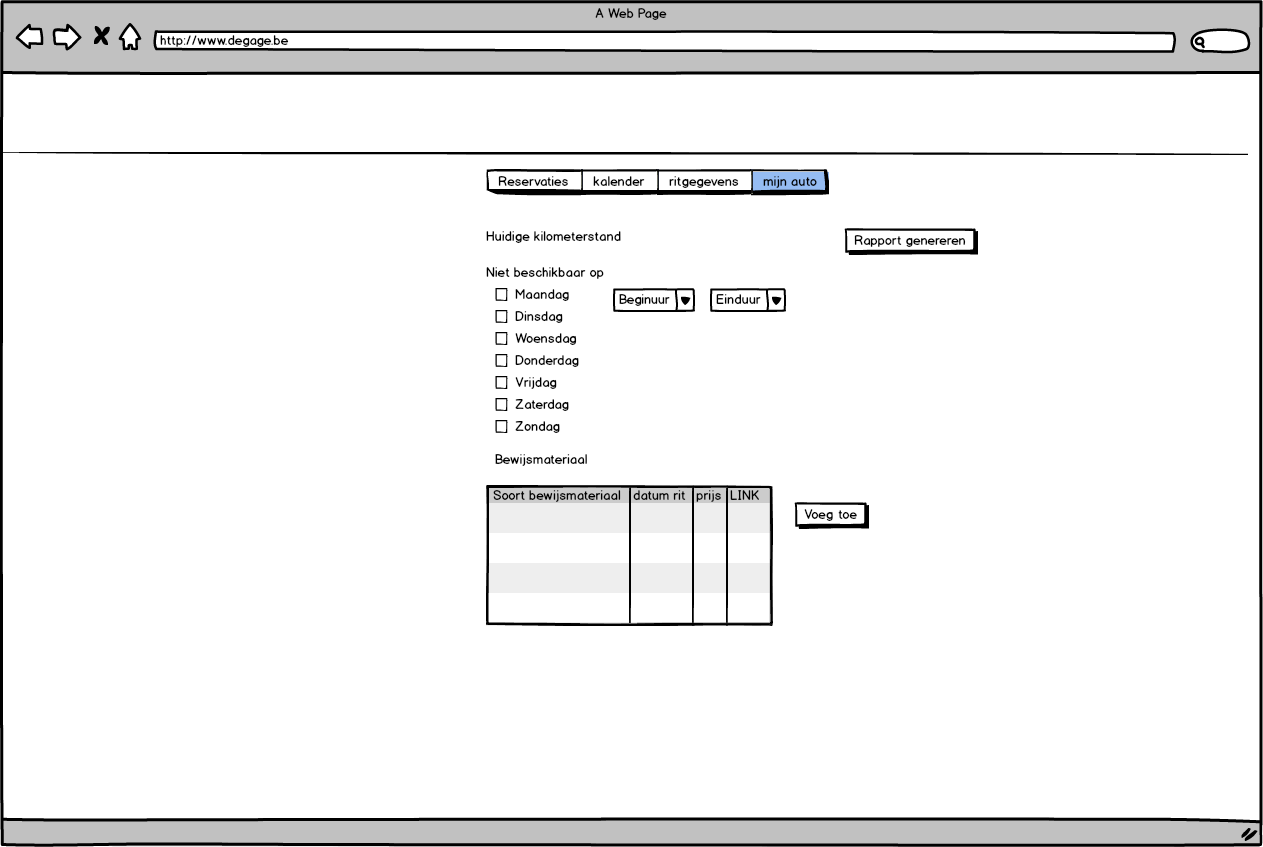
\includegraphics[width=\textwidth]{../../mockups/autobeheer_mijnauto.png}\end{figure}
\begin{figure}[H]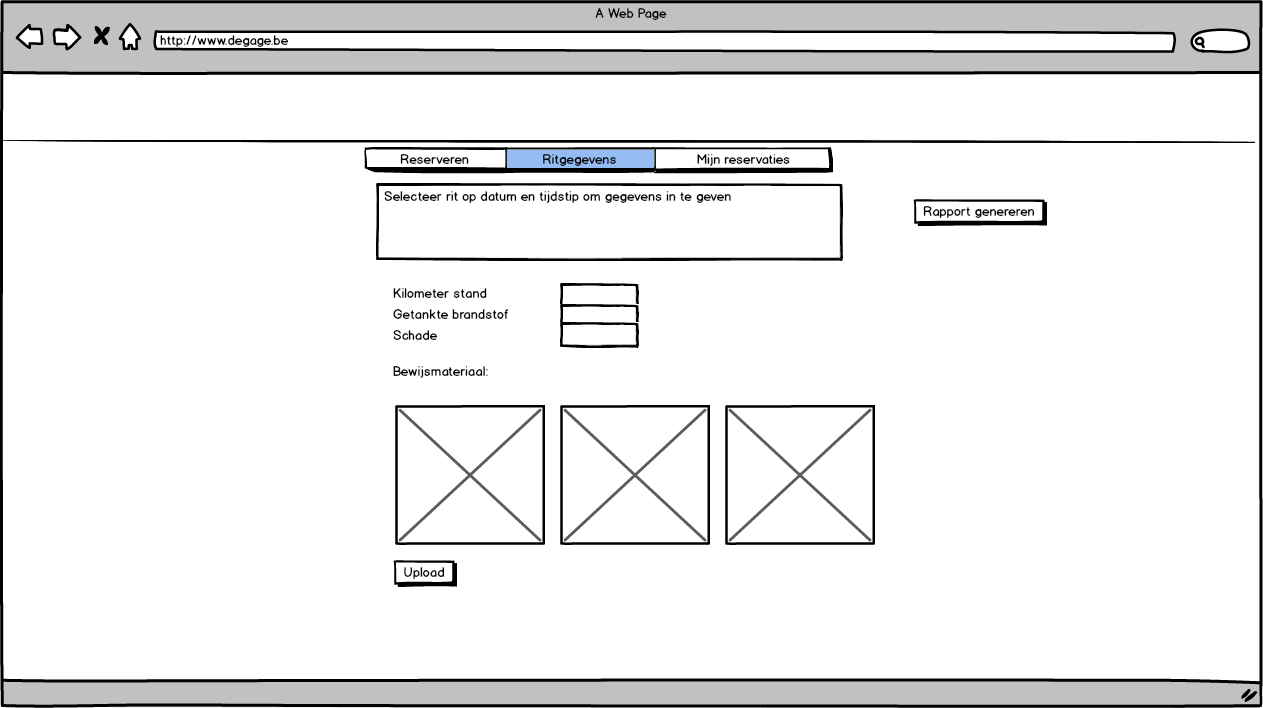
\includegraphics[width=\textwidth]{../../mockups/delen_ritgegevens.png}\end{figure}

\subsection{Goedkeuren of afkeuren van bewijsmateriaal}
\begin{figure}[H]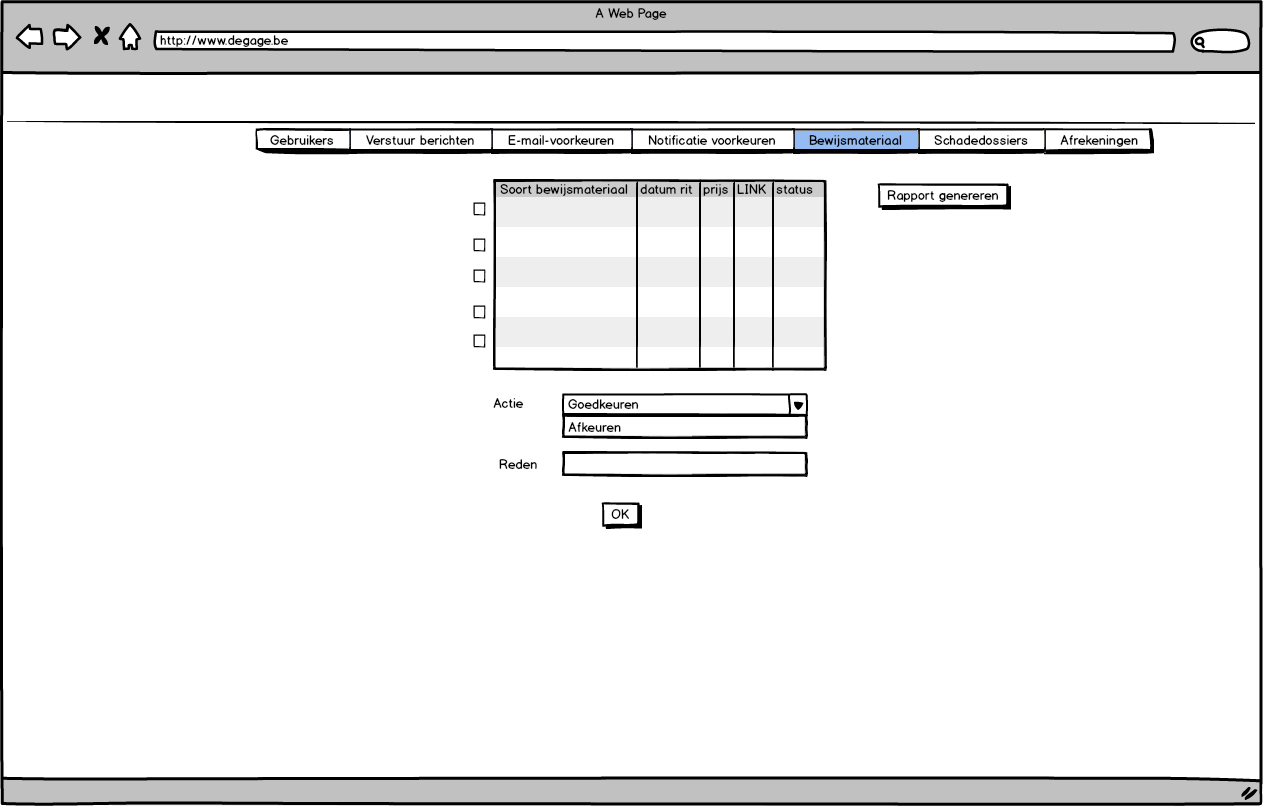
\includegraphics[width=\textwidth]{../../mockups/admin_verifierenbewijsmateriaal.png}\end{figure}

\setcounter{section}{0}
\setcounter{subsection}{0}
\part{Notificatiesysteem}
\section{Usescases}
\subsection{Ontvangen en bekijken van notificaties}
Bij bepaalde gebeurtenissen krijgt de gebruiker een notificatie (zoals bijvoorbeeld wanneer een door hem gemaakte reservatie wordt goedgekeurd).
Deze notificaties worden zowel op het dashboard (de homepage voor de gebruiker) getoond, als op een apart tabblad hiervoor. Het systeem is zeer goed
vergelijkbaar met het notificatiesysteem van facebook.

\subsection{Beheren van notificaties}
De beheerder kan bepalen bij welke gebeurtenissen er een notificatie moet gestuurd worden. Hiervoor is een aparte pagina voorzien.

\section{Mockups}
\subsection{Ontvangen en bekijken van notificaties}
\begin{figure}[H]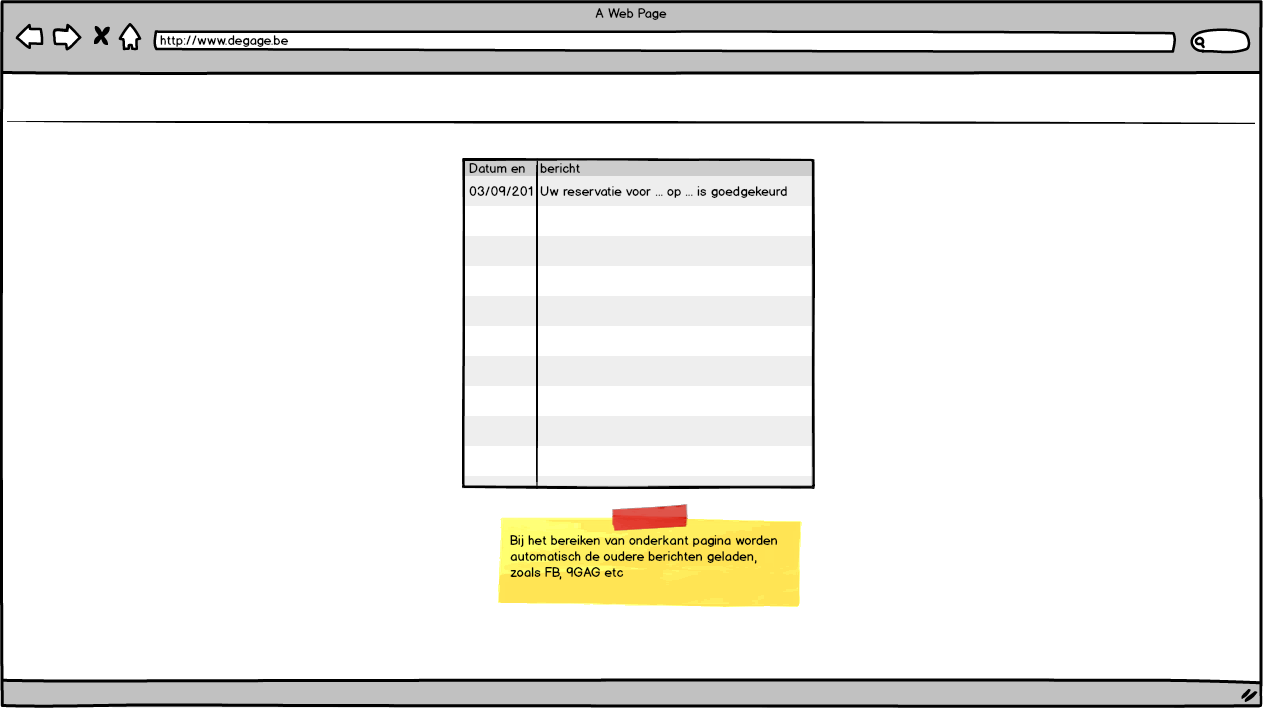
\includegraphics[width=\textwidth]{../../mockups/notificaties.png}\end{figure}

\subsection{Beheren van notificaties}
\begin{figure}[H]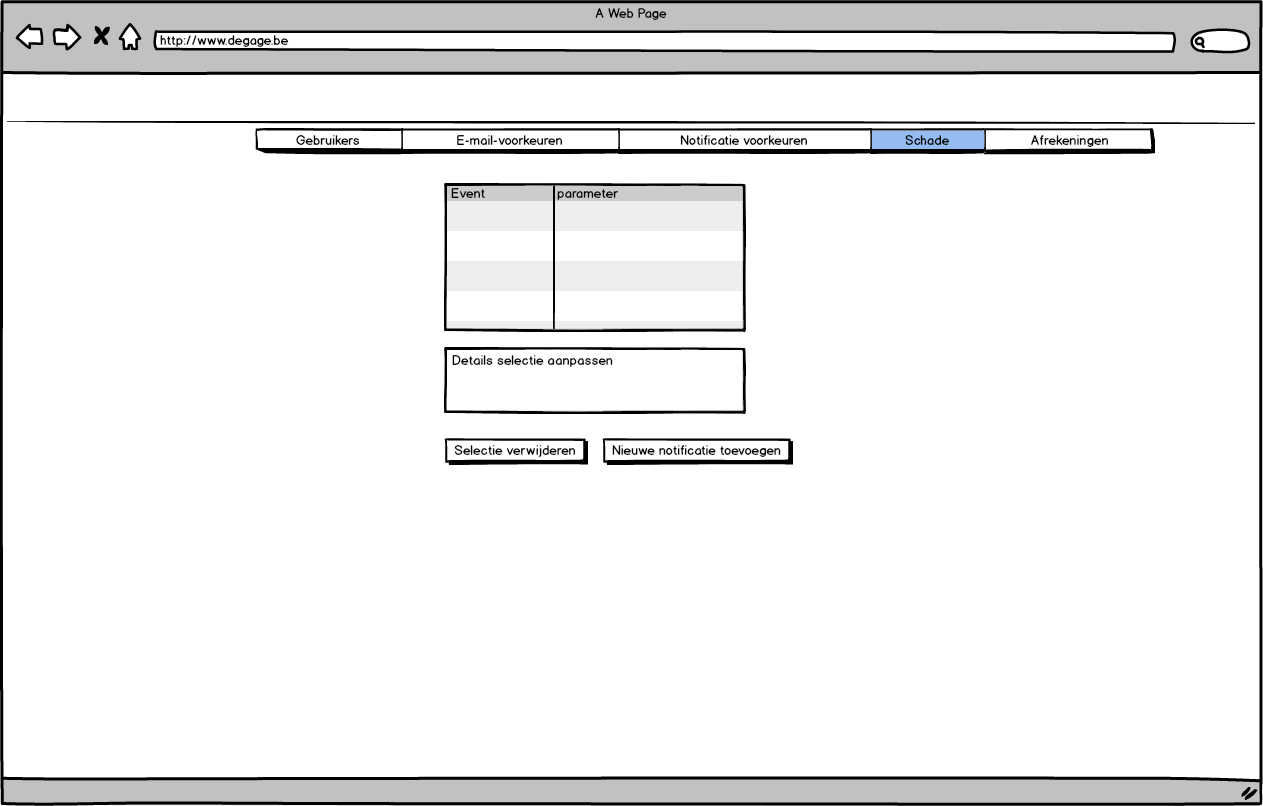
\includegraphics[width=\textwidth]{../../mockups/admin_notificatievoorkeuren.png}\end{figure}

\setcounter{section}{0}
\setcounter{subsection}{0}
\part{Rapportgeneratie}
\section{Usecases}
\subsection{Genereren van een rapport}
Waar mogelijk, wordt voor een beheerder een knop 'rapport genereren' voorzien. Als de gebruiker op die knop klikt, wordt een rapport gegeneerd
i.v.m de pagina waarop de beheerder zich op dat moment bevindt (bijvoorbeeld een bepaalde auto of gebruiker)

\section{Mockups}
\subsection{Genereren van een rapport}
\begin{figure}[H]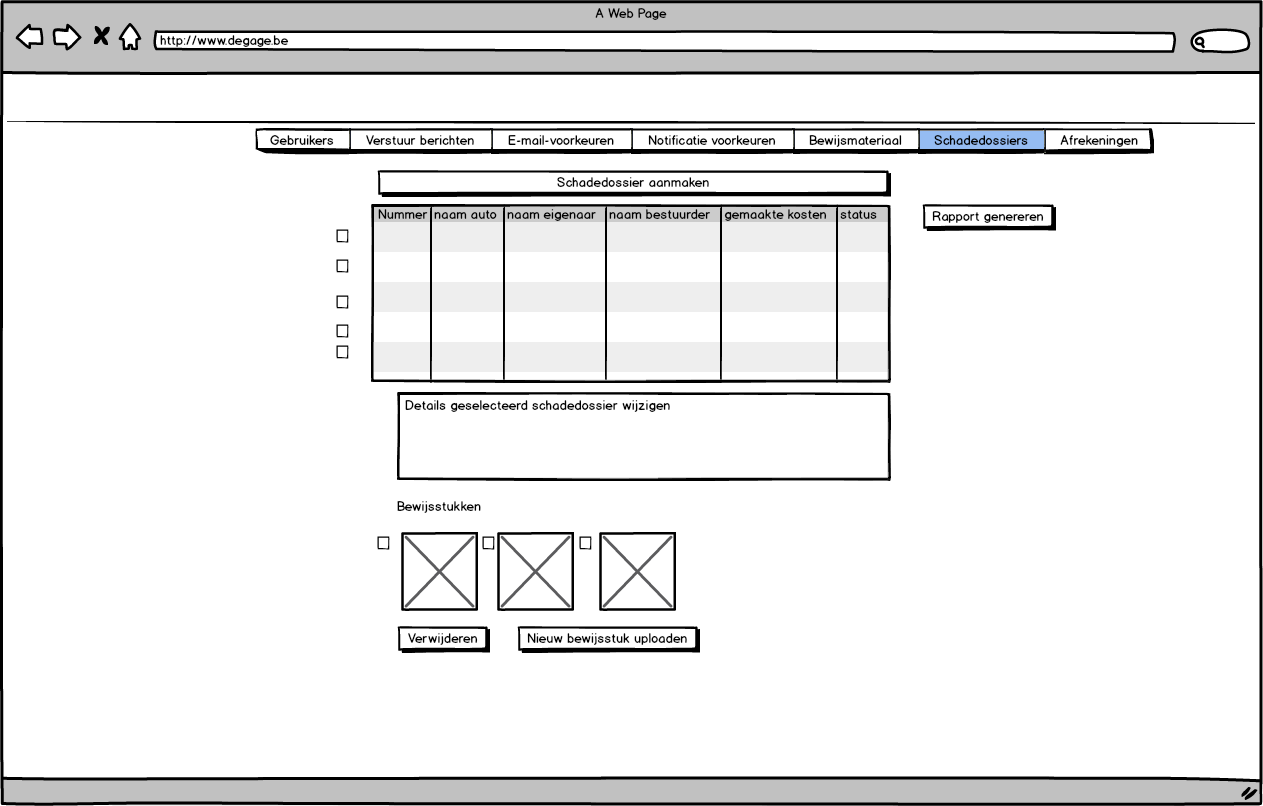
\includegraphics[width=\textwidth]{../../mockups/admin_schadedossiers.png}\end{figure}

\setcounter{section}{0}
\setcounter{subsection}{0}
\part{Schadedossiers}
\section{Usecases}
\subsection{Aanmaken van een schadedossier}
Voor het aanmaken en beheren van schadedossiers is een aparte pagina voorzien onder het tabblad 'Beheer'. Als een beheerder de machtiging heeft om
schadedossiers te beheren, kan hij een nieuwe aanmaken door op de gewenste knop te klikken. Hierbij moeten de volgende dingen meegegeven worden:
opmerkingen, bewijsstukken, status van het dossier (in behandeling, afgesloten, ...), naam van de auto, naam van de eigenaar,
naam van de bestuurder die de schade gemaakt heeft, gemaakte kosten, ...

\subsection{Wijzigen van een schadedossier}
Aan de hand van een zoekfunctie kan het gewenste schadedossier snel terug gevonden worden. Indien het gewenste schadedossier gevonden is,
kunnen de gewenste gegevens aangepast worden of dingen toegevoegd worden aan het dossier.

\section{Mockups}
\subsection{Aanmaken van een schadedossier}
\begin{figure}[H]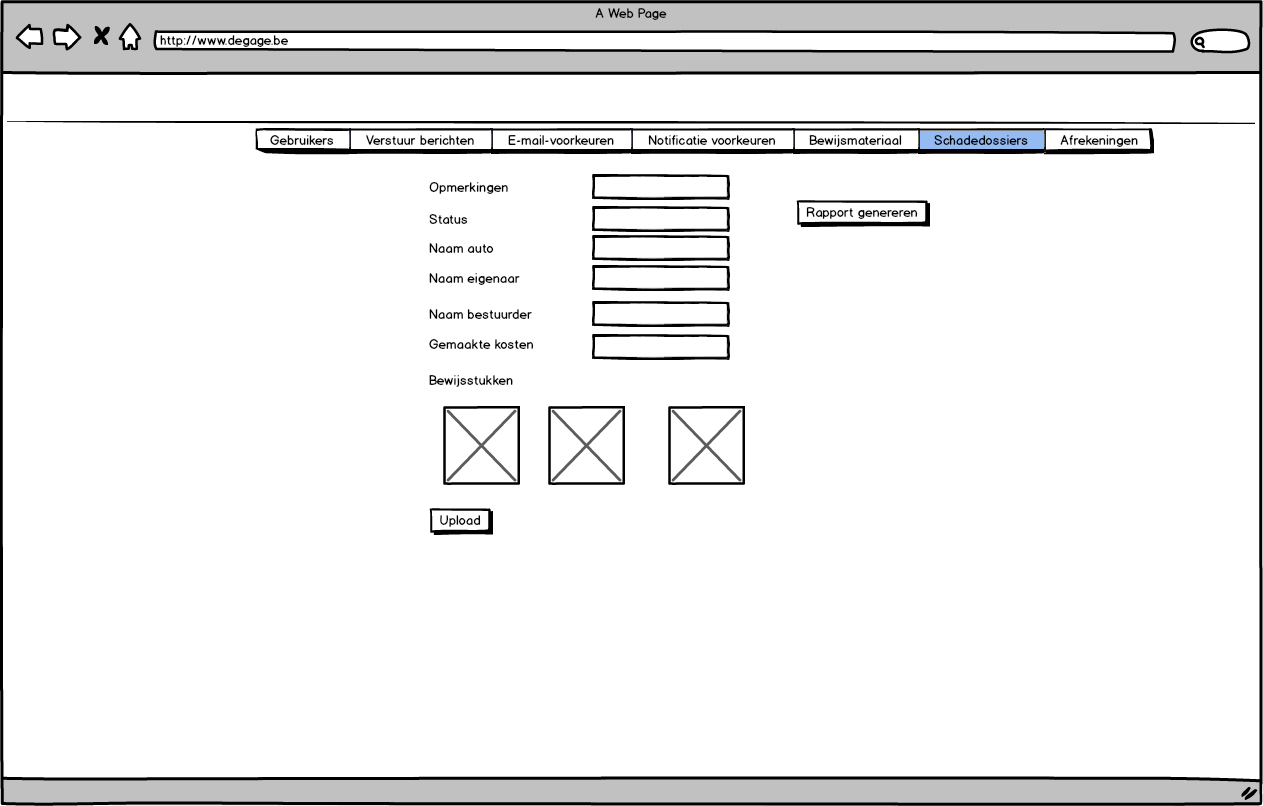
\includegraphics[width=\textwidth]{../../mockups/admin_schadedossiermaken.png}\end{figure}

\subsection{Wijzigen van een schadedossier}
\begin{figure}[H]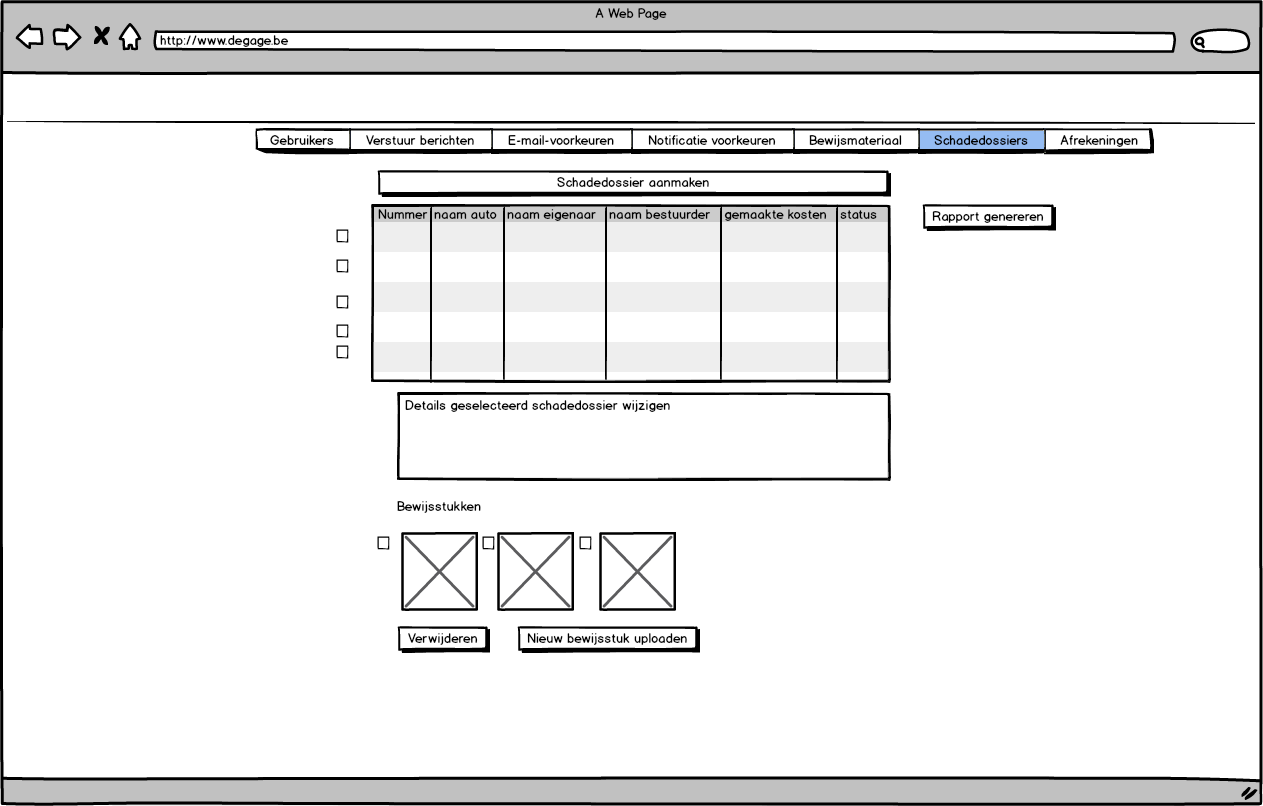
\includegraphics[width=\textwidth]{../../mockups/admin_schadedossiers.png}\end{figure}

\setcounter{section}{0}
\setcounter{subsection}{0}
\part{Tijdelijk blokkeren van een gebruiker}
\section{Usecases}
Indien een gebruiker zich niet aan de voorwaarden van de website houdt (bv. de gebruiker spamt), kan deze geblokkeerd worden. 
De beheerder selecteert de gewenste gebruiker, kiest voor 'blokkeer' en geeft een reden mee. Hierna wordt er een mail gestuurd naar de gebruiker in kwestie.

\section{Mockups}
\begin{figure}[H]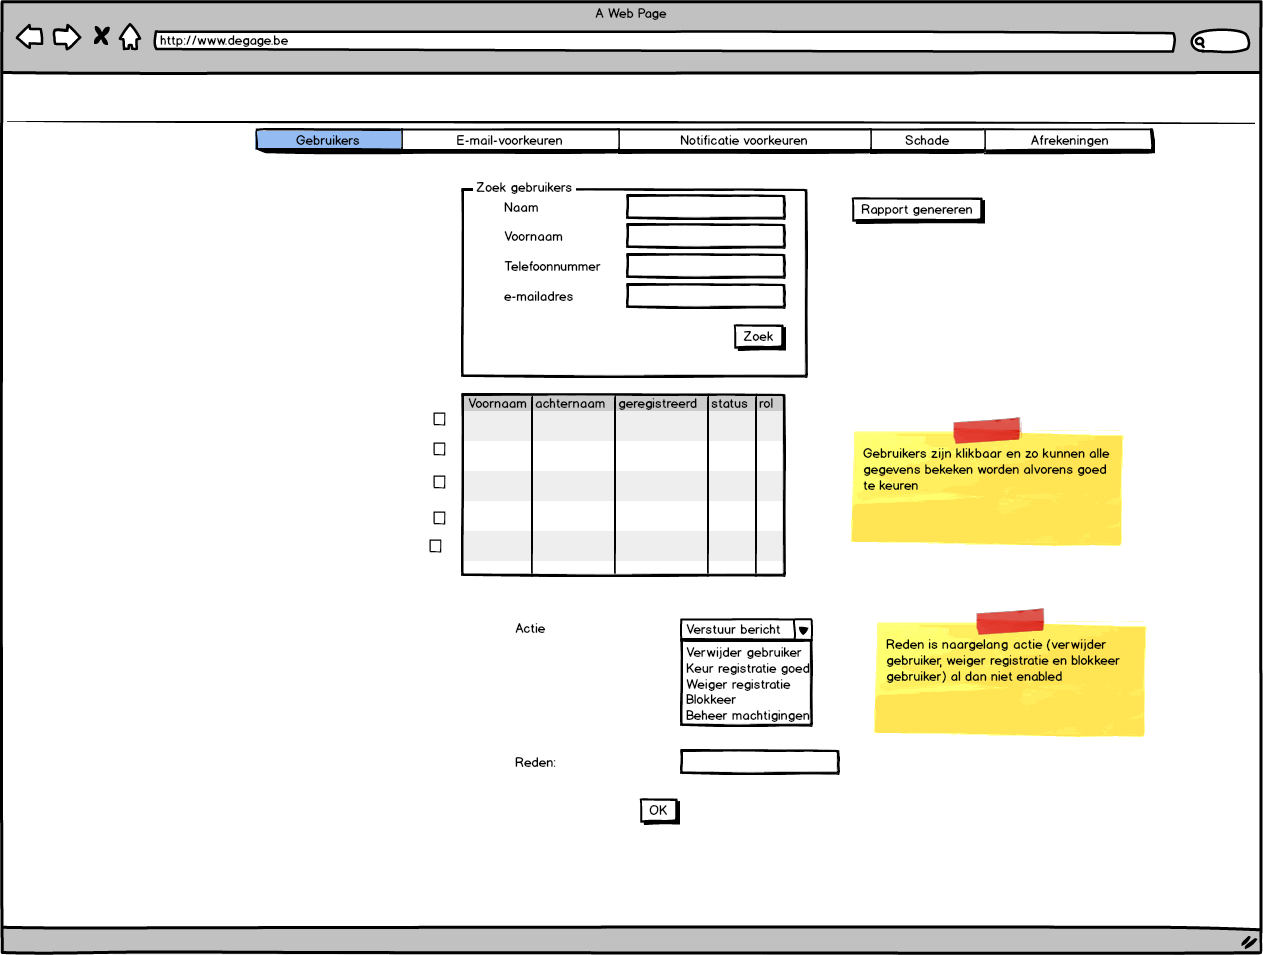
\includegraphics[width=\textwidth]{../../mockups/admin_dashboard_gebruikers.png}\end{figure}

\setcounter{section}{0}
\setcounter{subsection}{0}
\part{Machtigingen}
\section{Usescases}
Omdat we niet willen dat alle beheerders superusers zijn die alles kunnen, werken we met een machtigingensysteem. Elke taak van een beheerder
wordt geassocieerd met een machtiging. Een superuser kan dan machtigingen toekennen aan een bepaalde beheerder, of machtigingen afnemen.

\section{Mockups}
\begin{figure}[H]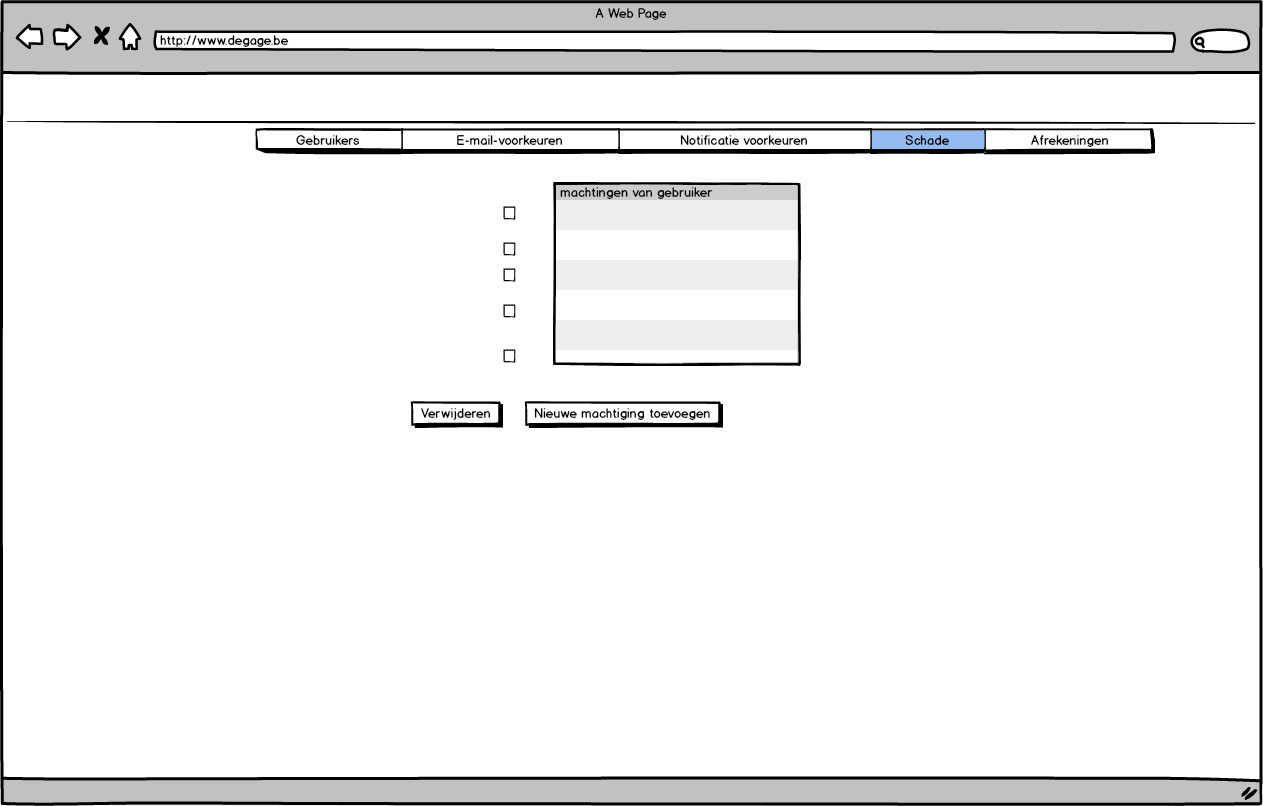
\includegraphics[width=\textwidth]{../../mockups/admin_machtigingentoevoegen.png}\end{figure}

\setcounter{section}{0}
\setcounter{subsection}{0}
\part{Autogebonden gegevens}
\section{Usescases}
Een autoeigenaar kan verschillende dingen van zijn auto bekijken. Zoals bijvoorbeeld een weekkalender om te zien wanneer zijn auto wel of niet
gereserveerd is. Ook kan de eigenaar autogebonden gegevens inbrengen, dit zijn gemaakte kosten zonder dat er een rit gedaan is (bv. onderhoud).

\section{Mockups}
\begin{figure}[H]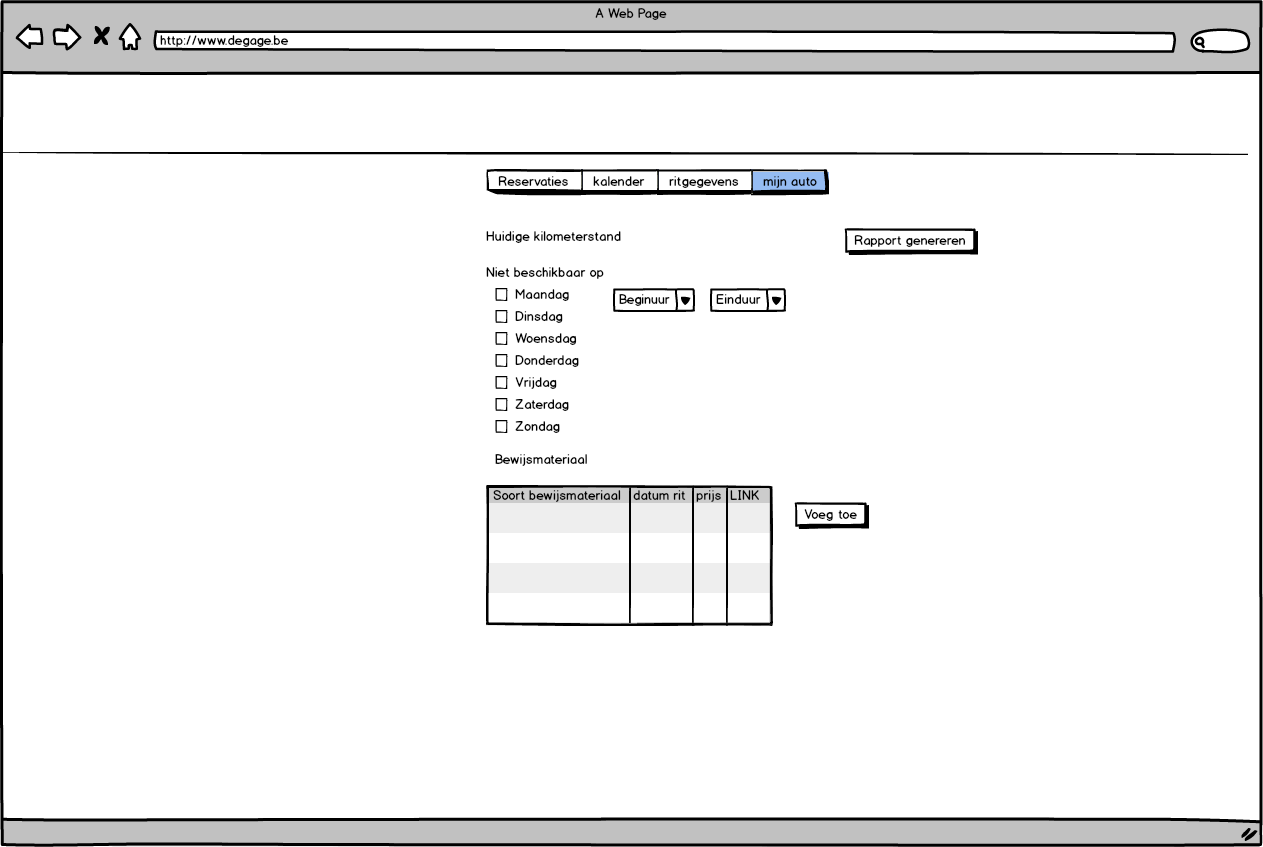
\includegraphics[width=\textwidth]{../../mockups/autobeheer_mijnauto.png}\end{figure}

\part{Inbrengen van nieuwe auto's}
\section{Usecases}
Bij de registratie van een autoeigenaar moeten de gegevens van zijn auto al ingebracht worden. De auto wordt wel niet rechtstreeks aan het
systeem toegevoegd, maar moet eerst goedgekeurd worden door een beheerder.

\section{Mockups}
\begin{figure}[H]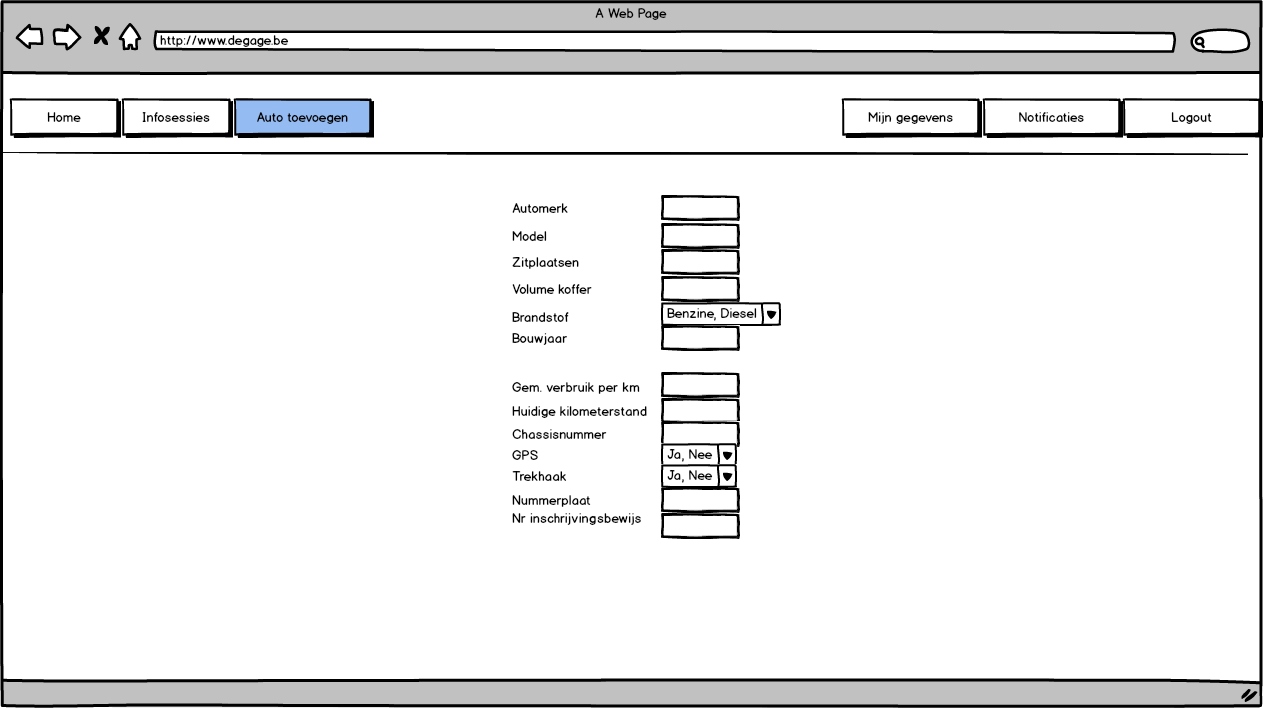
\includegraphics[width=\textwidth]{../../mockups/registratie_eigenaar_auto.png}\end{figure}
\begin{figure}[H]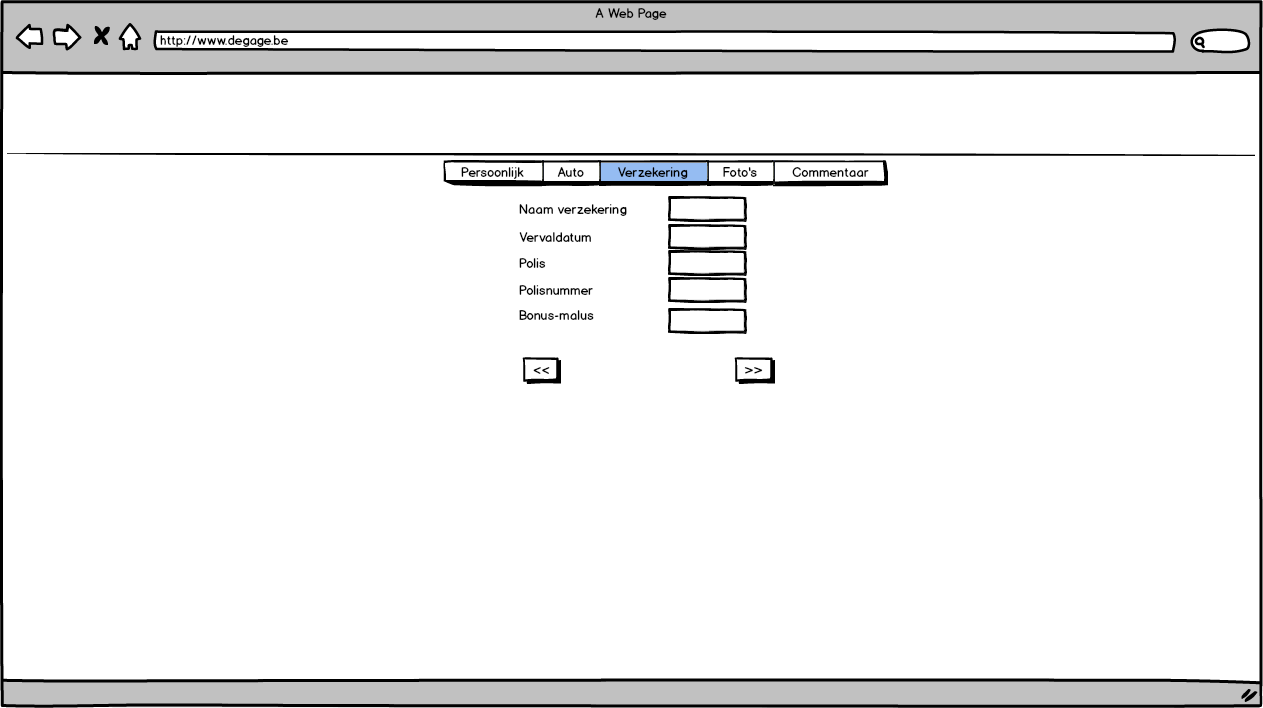
\includegraphics[width=\textwidth]{../../mockups/registratie_eigenaar_verzekering.png}\end{figure}
\begin{figure}[H]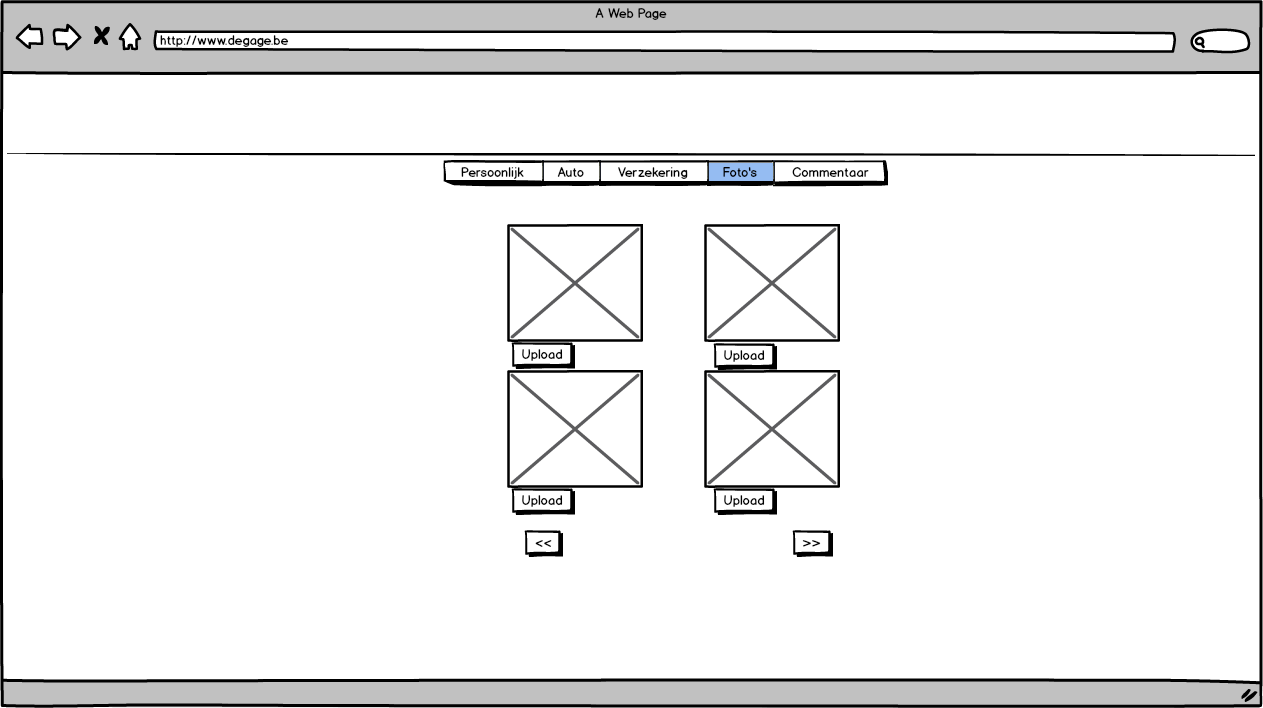
\includegraphics[width=\textwidth]{../../mockups/registratie_eigenaar_fotos.png}\end{figure}

\end{document}
